The line passes through
$\vec{a} = \myvec{1 \\2 \\-4}$

\begin{align}   
\vec{x} &=\myvec{ 8\\ -19\\ 10} + \lambda_1\myvec{ 3 \\-16\\ 7} \\
\vec{x} &=\myvec{15\\ 29\\ 5} + \lambda_2\myvec{ 3 \\8\\ -5} 
\end{align}


Let $\vec{n}$ be the normal vector to both lines. If $\vec{m_1}$ and $\vec{m_2}$ are the direction vectors of the lines,then
\begin{align}
\vec{m_1}^T  \vec{n} = 0 \\  
\vec{m_2}^T\vec{n} = 0    
\end{align}
Let the matrix $\vec{M}$ be
\begin{align}
\vec{M}=\myvec{\vec{m_1}^T\\\vec{m_2}^T}\\
\vec{m_1}=\myvec{3\\-16\\7} ,  \vec{m_2}=\myvec{3\\8\\-5},\vec{n}=\myvec{n_1\\n_2\\n_3} \\
\vec{M}\vec{n}=0
\end{align}
The matrix form is
\begin{align}
	\myvec{3 & -16 & 7 \\ 3 & 8 & -5}\\
	\myvec{3 & -16 & 7 \\ 3 & 8 & -5 } \xleftrightarrow{R_2=R_1-R_2}\myvec{3 & -16 & 7 \\ 0 & -24 & 12 }\\
	\myvec{3 & -16 & 7 \\ 0 & -24 & 12}\xleftrightarrow{R_2=\frac{R_2}{2}}\myvec{3 & -16 & 7 \\ 0 & -2 & 1 }\\
	\myvec{3 & -16 & 7 \\ 0 & -2 & 1 }\xleftrightarrow{R_1=R_1 -8R_2}\myvec{3 & 0 & -1 \\ 0 & -2 & 1}
\end{align}
We have 2 equations and 3 unknowns , we will have parametric solution
\begin{align}
 n_1 &=  \frac{k}{3}\\ n_2 &=  \frac{k}{2}\\ n_3 &= k \\
\vec{n} &= \frac{k}{6} \myvec{2 \\ 3 \\6}
\end{align}
The equation of required line is
\begin{align}
	\myvec{1\\2\\-4} + \lambda\myvec{2\\3\\6} 
\end{align}
See Fig.     \ref{fig:solutions/line_plane/1091}

\begin{figure}[!htbp]
    \centering
    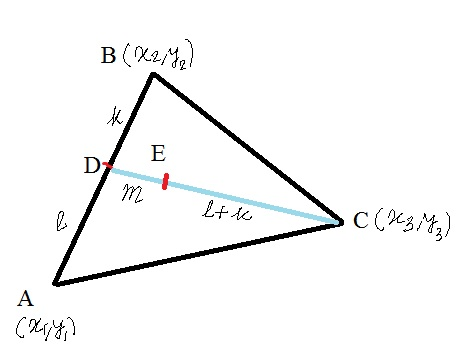
\includegraphics[width =\columnwidth]{./solutions/line_plane/109/assignment1.png}
    \caption{Perpendicular Line }
    \label{fig:solutions/line_plane/1091}
\end{figure}
